\icode[magenta]{N24E-MI-SI-L4-261108-001}
\nceeID[4]{2024湖北}{6}
如图所示，两拖船\(P\)、\(Q\)拉着无动力货船\(S\)一起在静水中沿图中虚线方向匀速前进，两根水平缆绳与虚线的夹角均保持为\qty{30}{\degree}。假设水对三艘船在水平方向的作用力大小均为\(f\)，方向与船的运动方向相反，则每艘拖船发动机提供的动力大小为\paren[]

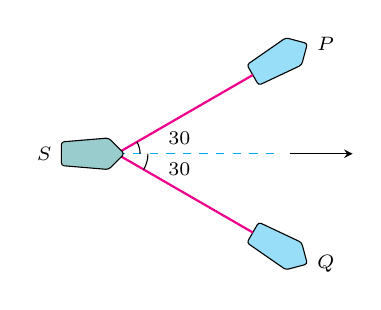
\begin{tikzpicture}[>=stealth,font=\scriptsize]
	\begin{scope}[rotate=30]
		\draw[fill=cyan!40,rounded corners=1] (2,.15)--(2.6,.2)--(2.8,0)node[right]{\(P\)}--(2.6,-.2)--(2,-.15)--cycle;
		\draw[thick,magenta] (0,0)--(2,0);
	\end{scope}
	\begin{scope}[rotate=-30]
		\draw[fill=cyan!40,rounded corners=1] (2,.15)--(2.6,.2)--(2.8,0)node[right]{\(Q\)}--(2.6,-.2)--(2,-.15)--cycle;
		\draw[thick,magenta] (0,0)--(2,0);
	\end{scope}
	\draw[dashed,cyan] (0,0)--(2,0);
	\draw (.3,0) arc(0:30:.3) (.4,0) arc(0:-30:.4);
	\draw[fill=teal!40,rounded corners=1] (.1,0)--(-.1,-.2)--(-.7,-.15)--(-.7,.15)--(-.1,.2)--cycle;
	\draw[->] (2.2,0)--(3,0);
	\node at(-.7,0)[left]{\(S\)};
	\node at(.8,.2){ \qty{30}{\degree}};
	\node at(.8,-.2){ \qty{30}{\degree}};
\end{tikzpicture}
\begin{choices}
	\item\(\frac{\sqrt{3}}{3}f\)
	\item\(\frac{\sqrt{21}}{3}f\)
	\item\(2f\)
	\item\(3f\)
\end{choices}
\begin{answer}
	B\qquad 提示：分解力，合成动力。
\end{answer}